\documentclass{amsart}
%\url{https://tex.stackexchange.com/q/438822/86}
\usepackage{tikz} 
\usetikzlibrary{positioning,knots}

\begin{document}

\[
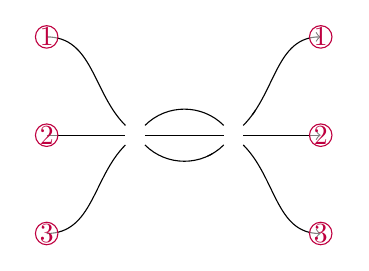
\begin{tikzpicture}

\node (KS1) at (0,0){};
\node (KS2) [below=1 of KS1]{};
\node (KS3) [below=1 of KS2]{};
\node (KC1) [right=1 of KS2] {};
\node (KC2) [right=1 of KC1] {};
\node (KT1) [above right=1 and 1 of KC2]{};
\node (KT2) [below=1 of KT1]{};
\node (KT3) [below=1 of KT2]{};

\begin{knot}[draft mode=crossings]
\strand[->] (KS1)
to [out=0, in=135] (KC1)
to [out=-45,in=-135] (KC2)
to [out=45, in=180] (KT1);
\strand[->] (KS2)
to [out=0, in=180] (KC1)
to [out=0, in=180] (KC2)
to [out=0, in=180] (KT2);
\strand[->] (KS3)
to [out=0, in=-135] (KC1)
to [out=45, in=135] (KC2)
to [out=-45, in=180] (KT3);
\redraw{1}{(KC2)}
\end{knot}

\end{tikzpicture}
\]

\end{document}

\documentclass{amsart}

\usepackage{tikz} 
\usetikzlibrary{positioning,knots}

\begin{document}

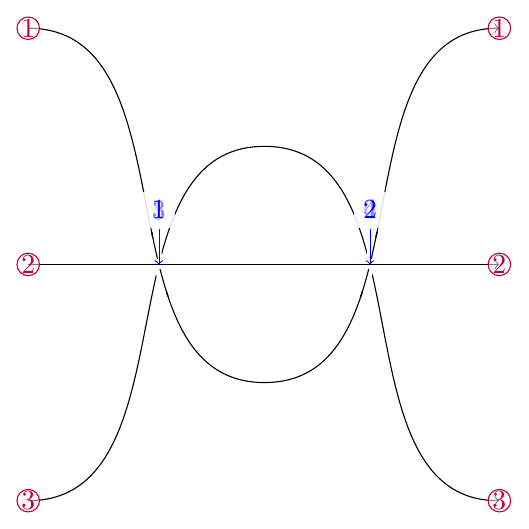
\begin{tikzpicture}[scale=3]
\begin{knot}[
  draft mode=crossings
]
\strand[->] (0,0) to[out=0,in=180] (1,-1.5) to[out=0,in=180] (2,0);
\strand[->] (0,-1) -- ++(2,0);% to[out=0,in=180] (1,-1) to[out=0,in=180] (2,-1);
\strand[->] (0,-2) to[out=0,in=180] (1,-.5) to[out=0,in=180] (2,-2);
%
% None: 3,1,2
% 2: 3,1,2
% 4: 1,3,2
% 6: 1,2,3
\end{knot}
\end{tikzpicture}

\vspace*{2cm}

%\[
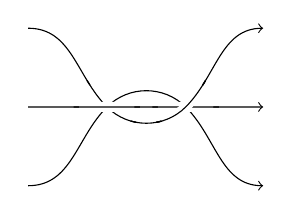
\begin{tikzpicture}[scale=3]

\coordinate (KS1) at (0,0){};
\coordinate [below=1 of KS1] (KS2){};
\coordinate [below=1 of KS2] (KS3){};
\coordinate [right=1 of KS2] (KC1) {};
\coordinate [right=1 of KC1] (KC2) {};
\coordinate [above right=1 and 1 of KC2] (KT1){};
\coordinate [below=1 of KT1] (KT2){};
\coordinate [below=1 of KT2] (KT3){};

  \begin{knot}[
%    draft mode=crossings,
%    ignore endpoint intersections=false
  ]
\strand[->] (KS1)
to [out=0, in=135] (KC1)
to [out=-45,in=-135] (KC2)
to [out=45, in=180] (KT1);
\strand[->] (KS2)
to [out=0, in=180] (KC1)
to [out=0, in=180] ([yshift=0cm]KC2)
to [out=0, in=180] (KT2);
\strand[->] (KS3)
to [out=0, in=-135] (KC1)
to [out=45, in=135] (KC2)
to [out=-45, in=180] (KT3);
\redraw{1}{(KC2)}
%\flipcrossings{2}%1,3,5,2}%,6,4,2}
\end{knot}

\end{tikzpicture}
%\]

\end{document}
